\documentclass[../main.tex]{subfiles}
\usepackage{silence}
\WarningFilter{glossaries}{No \printglossary or \printglossaries found}

\begin{document}
\ifSubfilesClassLoaded{%
	\graphicspath{{figures/4-AttOmics/}}%
	\setcounter{chapter}{3}%
}{
	\graphicspath{{../figures/4-AttOmics/}}%
}
\chapter{AttOmics}\label{chap:attomics}
\chapterpubli{attomics}
\minitocpage

\section{Model Architecture}
 \subsection{Architecture Details}
	 The model includes a grouping module and an encoder followed by a predictor, illustrated in \cref{fig:attomics_A}.
	 Instead of considering each feature individually, features are divided into different groups.
	 The encoder is a stack of $n$ blocks used to construct a new representation of the inputs.
	 Each block is formed of a \gls{gfcn} module where each group is projected into a lower dimension with a \gls{fcn}.
	 Segregating features in groups restrict the potential interactions between features to the ones inside the same group.
	 \Gls{mhsa} is applied to the set of groups to recover all possible interactions between groups.
	 Around the self-attention block, a residual connection is added before applying a normalization.
	 The encoder output is transmitted to an \gls{fcn} used as the predictor.

	 \begin{figure}[htbp]
		 \centering
		 \begin{subcaptiongroup}
			 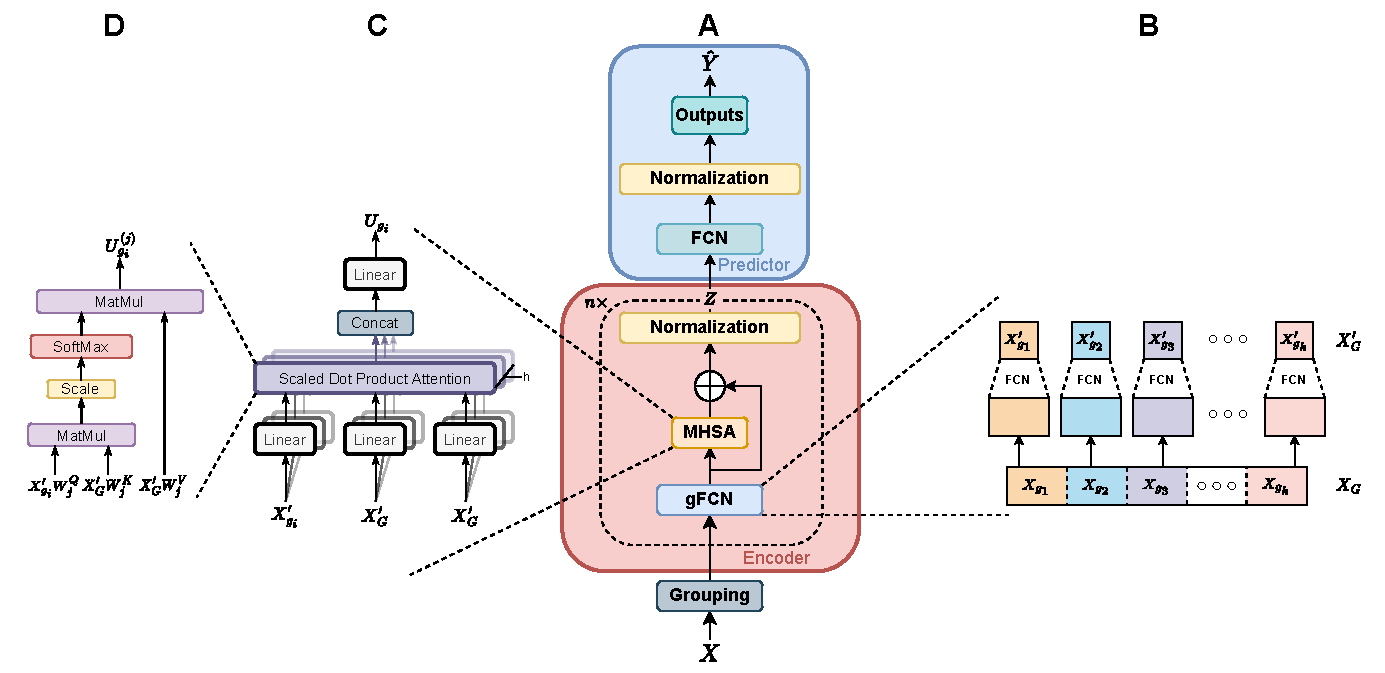
\includegraphics[width=\textwidth]{Beaude.168.fig.1.pdf}
			 \phantomcaption\label{fig:attomics_A}
			 \phantomcaption\label{fig:attomics_B}
			 \phantomcaption\label{fig:attomics_C}
			 \phantomcaption\label{fig:attomics_D}
		 \end{subcaptiongroup}
		 \caption[The AttOmics architecture]{The AttOmics architecture is composed of a grouping module, an encoder and a predictor~\subref{fig:attomics_A}. The grouping module transforms the input features into a set of different groups. In each of the $n$ encoder blocks, each group is projected into a lower dimensional space~\subref{fig:attomics_B}. Interactions between the different groups is computed with the \glsfirst{mhsa}~\subref{fig:attomics_C}. In each of the $h$ heads of the \gls{mhsa}, a scaled-dot product attention is computed between the different groups~\subref{fig:attomics_D}. A residual connection is added around the \gls{mhsa} before applying a normalization. The new representation obtained with the encoder is transmitted to the predictor, a \glsfirst{fcn} followed by a normalization.~\subrefrange{fig:attomics_A}{fig:attomics_C}}\label{fig:attomics_arch}
	 \end{figure}

	 \subsubsection{Grouped FCN (gFCN)}
		 Let $X \in \mathbb{R}^p$ be a training example where $p$ is the number of features and $Y$ is the associated label.
		 The training example $X$ is split into groups according to a grouping strategy (see \cref{sec:grouping}), $ X_G = \left\{X_{g_i} \right\}_{1 \leq i \leq k}$, where $k$ is the number of groups.
		 For each group  $X_{g_i}$, a group embedding is independently computed as $X_{g_i}'$ by projecting it into an $s$-dimensional space with an \gls{fcn}, a succession of \glspl{fcl}~(\cref{fig:attomics_B}).

		 Each \gls{fcl} is the composition of an affine transformation of its inputs with a \gls{relu} activation function:
		 \[ \operatorname{FCL}\left(x\right) = \operatorname{ReLU}\left(Wx+b \right) = \max\left(0, Wx+b\right) \]

		 After processing each group $X_{g_i}$ by the successive \gls{fcl}, we obtain the set of group embeddings $X'_G$:
		 \[ X_G' = \left\{ X_{g_i}' \in \mathbb{R}^{s}\right\}_{1 \leq i \leq k} \text{,} \]
		 where $X_{g_i}' = \operatorname{FCN}\left(X_{g_i}\right)$.

		 Each group projection is only computed using elements from the same group.
		 To create a representation of the expression vector based on all possible interactions, \gls{mhsa} is then applied to $X'_G$.

	 \subsubsection{Multi-Head Self-Attention}

		 \Gls{mhsa} is applied to construct a new representation of the groups, \(U = \left\{ U_{g_i}\right\}_{1 \leq i \leq k}\), by allowing them to interact with each other~(\cref{fig:attomics_C}).

		 \Gls{mhsa} is performed with $h$ different heads to learn different types of interactions.
		 For each head $j$, self-attention is applied to each group $g_i$~($1 \leq i \leq k $), in order to obtain: $U^{(j)} = \left\{ U^{(j)}_{g_i} \in \mathbb{R}^{l} \right\}_{1 \leq i \leq k}$, where $l = \frac{s}{h} \in \mathbb{N}$.

		 $U^{(j)}_{g_i}$ is defined by:

		 \[ U^{(j)}_{g_i} = A^{(j)}_{g_i} \cdot \left[ X_{g_1}' \cdot W_j^V, \ldots ,  X_{g_k}' \cdot W_j^V\right]^T \text{,}\]

		 where $A^{(j)}_{g_i}$ is the attention vector computed by the usual dot product attention~(\cref{fig:attomics_D})~\cite{vaswaniAttentionAllYou2017}:

		 \begin{align*}
			 A^{(j)}_{g_i}      & = \operatorname{softmax}\left(\left[A^{(j)}_{g_i,g_1}, \ldots,  A^{(j)}_{g_i,g_k}\right]\right) \text{,}  \\
			 A^{(j)}_{g_i, g_k} & =  \frac{\left(X_{g_i}' \cdot W_j^Q\right)^T \cdot \left(X_{g_k}' \cdot W_j^K \right)}{\sqrt{s}} \text{.}
		 \end{align*}

		 Projection matrix $W^Q_j$ (respectively $W^K_j$ and $W^V_j$) maps the group $X_{g_i}'$, from an $s$-dimensional space to an $l$-dimensional space.
		 In the transformers formulation $X_{g_i}' \cdot W_j^Q$, $X_{g_k}' \cdot W^K_j$, and $X_{g_i}' \cdot W^V_j$ are called, query, key, and value respectively.

		 Each element of $U_{g_i}$ is obtained by concatenating the representation of all groups in the different heads and projecting each group to an $s$-dimensional space using a projection matrix $W^O \in \mathbb{R}^{s\times s}$ as:
		 \[ U_{g_i} = \operatorname{concat}\left( U^{(1)}_{g_i}, \ldots, U^{(h)}_{g_i} \right) \cdot W^O \text{,}\]
	 \subsubsection{Residual connection and normalization}
		 The value of $X_{g_i}'$ is added to $U_{g_i}$, through a residual connection to prevent vanishing gradients.\\
		 The last step in the encoder module consists of applying a normalization to obtain the final representation $Z_{g_i}$ of group $g_i$ defined as:

		 \[Z_{g_i} = \operatorname{Norm}\left(X_{g_i}' + U_{g_i} \right) \text{.}\]

		 The output of an encoder block is $Z = \left\{ Z_{g_i} \in \mathbb{R}^{s}\right\}_{1 \leq i \leq k}$, which is a representation of the groups capturing their interactions.

	 \subsubsection{Prediction module}
		 The vectors $Z_{g_i}$ are concatenated into a new vector $Z' \in \mathbb{R}^{ks}$.
		 The output of the encoder $Z'$ is then fed to a \gls{fcn} followed by a normalization layer to predict the cancer type or the prognosis $\hat{Y}$~(\cref{fig:attomics_A}).

		 For classification tasks,  the output layer has one neuron per class, and a $\operatorname{softmax}$ activation function is applied to get the probability vector \(P = \left[p_c\right]_{1\leq c\leq M}\), where $M$ denotes the number of classes.
		 For the survival analysis, the output is a single neuron with a linear activation function.

 \subsection{Grouping strategies}\label{sec:grouping}

	 The AttOmics architecture can be applied to any group specification.
	 We explore different grouping strategies such as random groups, groups obtained with clustering, groups based on biological information like the \gls{go}~\cite{geneontologyconsortiumGeneOntologyResource2021} or the hallmarks collection available in MSigDB~\cite{Liberzon2015}.

	 \begin{description}[
			 style=multiline,
			 leftmargin=!,
			 labelwidth=\eqboxwidth{listlabel@\EnumitemId}, format=\mylabelformat
		 ]
		 \item[Random] With the random strategy, groups are formed by randomly sampling the input features in groups of similar sizes, $p/k$.
		 \item[Gene Ontology] We used \gls{bp} gene-ontology as it groups different molecular activities in a shared process which are more likely linked to the same cancer phenotype.
		       To avoid possible problems with selecting the \gls{go} terms (i.e.\ groups) of interest, we restrict ourselves to terms available in \gls{go} slims.

		       Inside the \gls{bp} slim ontology, a gene can belong to more than one group; on average, they belong to two groups.
		       Before applying self-attention, each group must be projected into the same dimensional space.
		       Each group is projected with a different number of layers to have the same reduction ratio across different groups. This grouping strategy can only be applied to \gls{mrna} data.
		 \item[Hallmarks] In the MSigDB hallmarks collection~\cite{Liberzon2015}, there are 50 groups.
		       Each one represents a well-defined biological process.
		       Each group is projected with a different number of layers to ensure identical reduction ratio across different groups. This grouping strategy can only be applied to \gls{mrna} data.
		 \item[Clustering]The clustering strategy groups features based on their expression levels.
		       Traditional clustering methods, like K-Means or hierarchical clustering, can return sets of highly unbalanced clusters that may negatively affect the efficiency of our model.
		       Large groups would require many parameters to be projected into a space with a dimension lower than the smallest group.
		       Group unbalances would also imply a high compression of larger groups and almost no compression for the smallest group.
		       To prevent this, we used constrained K-means clustering to ensure comparable group sizes~\cite{bradleyConstrainedKMeansClustering}.
	 \end{description}


 \subsection{Model training}

	 For classification problems, our model is trained end-to-end with a weighted cross-entropy loss to account for class imbalance:
	 \[ \mathcal{L}(\theta) = - \sum_{c=1}^{M}w_c Y_c \log\left( p_c\right) \text{,}\]
	 where $w_c$ denotes the weight (inversely proportional to the size) of class $c \in \left\{1, \ldots,M \right\}$ and $\theta$ the model parameters.

	 For survival analysis, our model is end-to-end trained with a partial log-likelihood loss, as proposed in DeepSurv~\cite{katzmanDeepSurvPersonalizedTreatment2018}:
	 \[ \mathcal{L}(\theta) = \frac{1}{N_{\delta_i = 1}} \sum_{i:\delta_i=1} \left(\hat{Y}_i - \log \sum_{j \in \mathcal{R}(T_i)}\eta_j \right) \text{,}\]
	 where $\delta_i$ specifies if the event occurred for patient $i$, $T_i$ represents the time associated to the event and $N_{\delta_i = 1}$ is the number of patients for which the event occurred ($\delta_i = 1$).
	 $\eta_i = e^{\hat{Y}_i}$ is the predicted risk for patient $i$.
	 $\mathcal{R}(T_i) = \{j: T_j > T_i\}$ is the risk set, the set of patients who are still at risk of death at time $T_i$.

\section{Experiments}
 \subsection{Data}

	 TCGA data were used to evaluate our proposed approach AttOmics.
	 We collected DNA methylation, gene expression, and miRNA expression data for 8416 patients of 19 different cancers and 361 normal samples from the GDC Data Portal\footnote{\url{https://portal.gdc.cancer.gov/}}.
	 FFPE samples and bad replicates were removed according to TCGA consortium recommendation.
	 Methylation data was restricted to the probes common to both HumanMethylation27 and HumanMethylation450 platforms.
	 No feature selection was applied, and data were standardized to a zero mean and unit variance.

	 Patients with incorrect survival information were removed: 8349 patients were available for survival prediction.
	 70\% of the data is used as a training set, 15\% forms the validation set, and the remaining 15\% forms the test set while preserving the proportion of each cancer.

	 The training set is used to perform two predicting tasks: phenotype prediction, 19 different cancers and normal, and survival risk prediction.

 \subsection{Comparative study}
	 For a comprehensive and comparative evaluation, we choose three deep learning architectures for comparison: \gls{cnn}, \gls{gnn}, and \gls{mlp}.

	 For the \gls{cnn} (CNN1d), we ordered features based on their position on the genome, then used a 1D convolution, followed by a \gls{relu} activation and a maximum pooling.
	 For the \gls{gnn} architecture, two graphs were used: \gls{ppi} (GNN --- PPI) and co-expression (GNN --- CoExp) graphs.
	 The \gls{ppi} graph is based on data available in the STRING database~\cite{Szklarczyk2020} and was constructed by retaining only high-confidence links: edges with a score higher than 700.
	 The co-expression graph was constructed similarly to~\cite{ramirezClassificationCancerTypes2020}.
	 The Spearman correlation matrix between gene expressions was computed.
	 If the correlation was higher than a threshold and the associated p-value was lower than 0.05, then an edge between the two features was added to the graph.
	 For \gls{mrna} and \gls{mirna}, the correlation threshold was set to 0.6.
	 For \gls{dnam} a 0.7 correlation threshold was used.
	 Self-loops were not considered in the graph construction, and isolated nodes were removed.
	 The \gls{ppi} graph and the co-expression graph for \gls{mrna} have 9384 genes in common.
	 Each graph is described in the supplementary file~(Table S2).
	 \Gls{mlp} architecture has two hidden layers with \gls{relu} activation and makes use of batch normalization.
	 We also consider three state-of-the-art non-deep-learning models for comparison: \gls{svm}, \gls{rf}, and \gls{xgboost}.
	 For the non-deep-learning approaches, the 2000 most discriminative features are selected with a t-test-based selection.

	 The hyper-parameters of each approach are tuned on each omics data with a random search to achieve the best performances.
	 The different values tested for each parameter are defined in the supplementary material (Table S3).
	 For each hyper-parameter at each search iteration, a value is randomly drawn from the defined range.
	 A model is constructed using these parameters, trained on the training set, and evaluated on the validation set.
	 The selected hyper-parameters for each architecture are presented in the supplementary file~(Table S5).

	 AttOmics is trained end-to-end using the Adam optimizer with a learning rate of 0.0001 and a batch size of 512.
	 The maximum number of epochs was set to 100.
	 An early stopping strategy is deployed to avoid over-fitting with a patience of 8 and a delta of 0.001 on the validation metric between two epochs.

	 For the classification task, models were evaluated with the error rate.
	 Prognosis prediction is evaluated with the concordance index~\cite{harrellMultivariablePrognosticModels1996}.
	 It estimates that for a pair of individuals, the predicted risks, $\eta$,  are concordant with their actual survival times.
	 \[ \operatorname{C-Index} = \frac{\sum_{i,j}\mathbb{1}_{T_j < T_i}\mathbb{1}_{\eta_j > \eta_i}\delta_j}{\sum_{i,j}\mathbb{1}_{T_j < T_i}\delta_j} \]
	 A $\operatorname{C-Index} = 0.5$ represents a random prediction and $\operatorname{C-Index} = 1$ corresponds to a perfect ranking.
	 Results for the prognosis task are presented in the supplementary.

\section{Results}

 \subsection{Hyper-parameters choice}

	 We investigate the impact of the main hyper-parameters on the model error rate by applying a random search procedure.
	 For each hyper-parameter, a random value is drawn from a set of predefined possible values.
	 A model is trained with selected hyper-parameters on the training dataset.
	 For each grouping strategy, 1500 models are trained.
	 The performance metrics reported here are estimated on the validation set.
	 The results for the main hyper-parameters of this experiment are presented in \cref{fig:hparams_search}.
	 The performance obtained for each tested value is represented with a boxplot.

	 \begin{figure}[htbp]
		 \centering
		 \begin{subcaptiongroup}
			 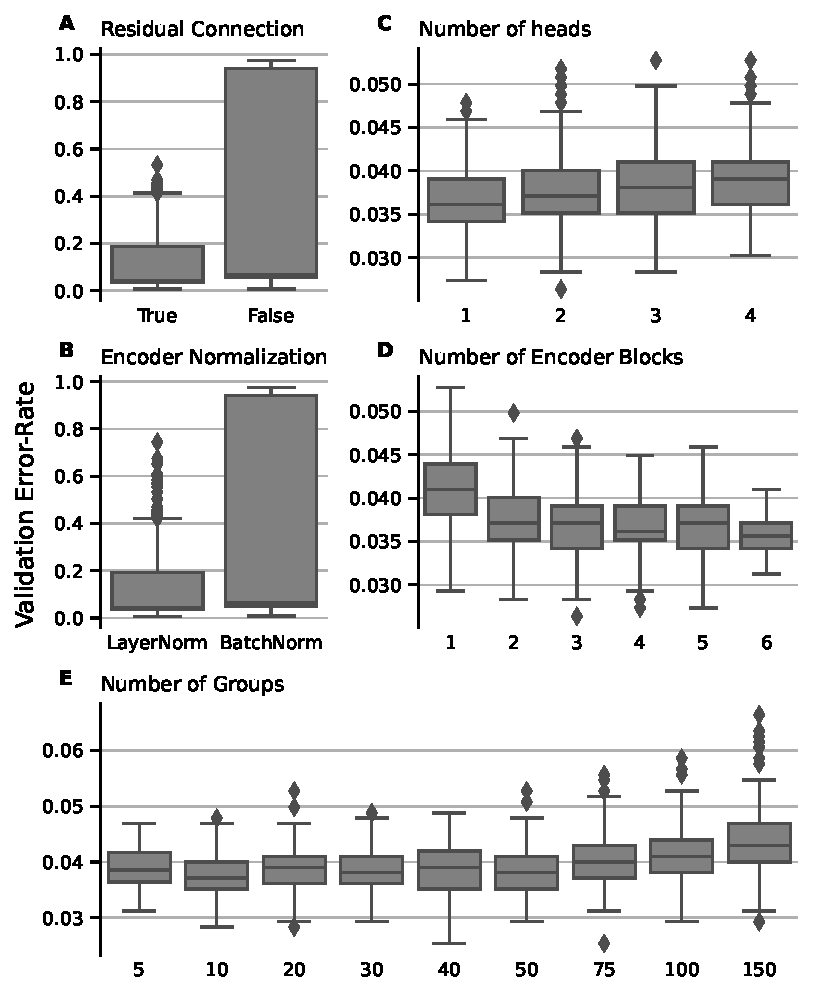
\includegraphics[width=0.9\linewidth]{Beaude.168.fig.2.pdf}
			 \phantomcaption\label{fig:attomics_hparams_search_A}
			 \phantomcaption\label{fig:attomics_hparams_search_B}
			 \phantomcaption\label{fig:attomics_hparams_search_C}
			 \phantomcaption\label{fig:attomics_hparams_search_D}
			 \phantomcaption\label{fig:attomics_hparams_search_E}
		 \end{subcaptiongroup}
		 \caption{Results of the random search for \gls{mrna} data with the clustering grouping strategy}\label{fig:hparams_search}
	 \end{figure}

	 The encoder's residual connection and the choice of normalization type greatly impact the performances.
	 Adding a residual connection in an encoder block significantly impacts the model's performance.
	 It stabilizes the model performances~(\cref{fig:attomics_hparams_search_A}).
	 We explore two types of normalization in the encoder: layer normalization (LayerNorm) and batch normalization (BatchNorm).
	 Layer normalization gives better and more stable results (\cref{fig:attomics_hparams_search_B}).
	 The different hyper-parameters which control the model architecture impact the performances differently.
	 A sufficient number of encoder blocks is required to achieve the best performances.
	 There is an 11\% error rate improvement from 1 to 3 blocks.
	 Beyond three blocks, there is no error rate decrease (\cref{fig:attomics_hparams_search_D}).
	 The number of heads used in the \gls{mhsa} layer has no significant impact on the validation error rate.
	 There is only a 0.002 mean validation error rate difference between 1 and 4 heads (\cref{fig:attomics_hparams_search_C}).

	 Another important hyper-parameter of the architecture is the number of groups (\cref{fig:attomics_hparams_search_E}).
	 An increase in the number of groups impacts the model performances.
	 There is a 10\% increase in the error rate between 10 and 100 groups.
	 In the range of 10 to 50 groups, the impact on the performances is limited.
	 The maximum mean error rate difference observed is 0.004, which is less than 1\% of variation.
	 Increasing the number of groups also impacts the model complexity as self-attention scales quadratically with the number of groups.

	 The selected hyper-parameters for each grouping strategy and each omics data are presented in the supplementary file (Table S4).

 \subsection{Comparison with state of the art}

	 \begin{figure*}[htbp]
		 \centering
		 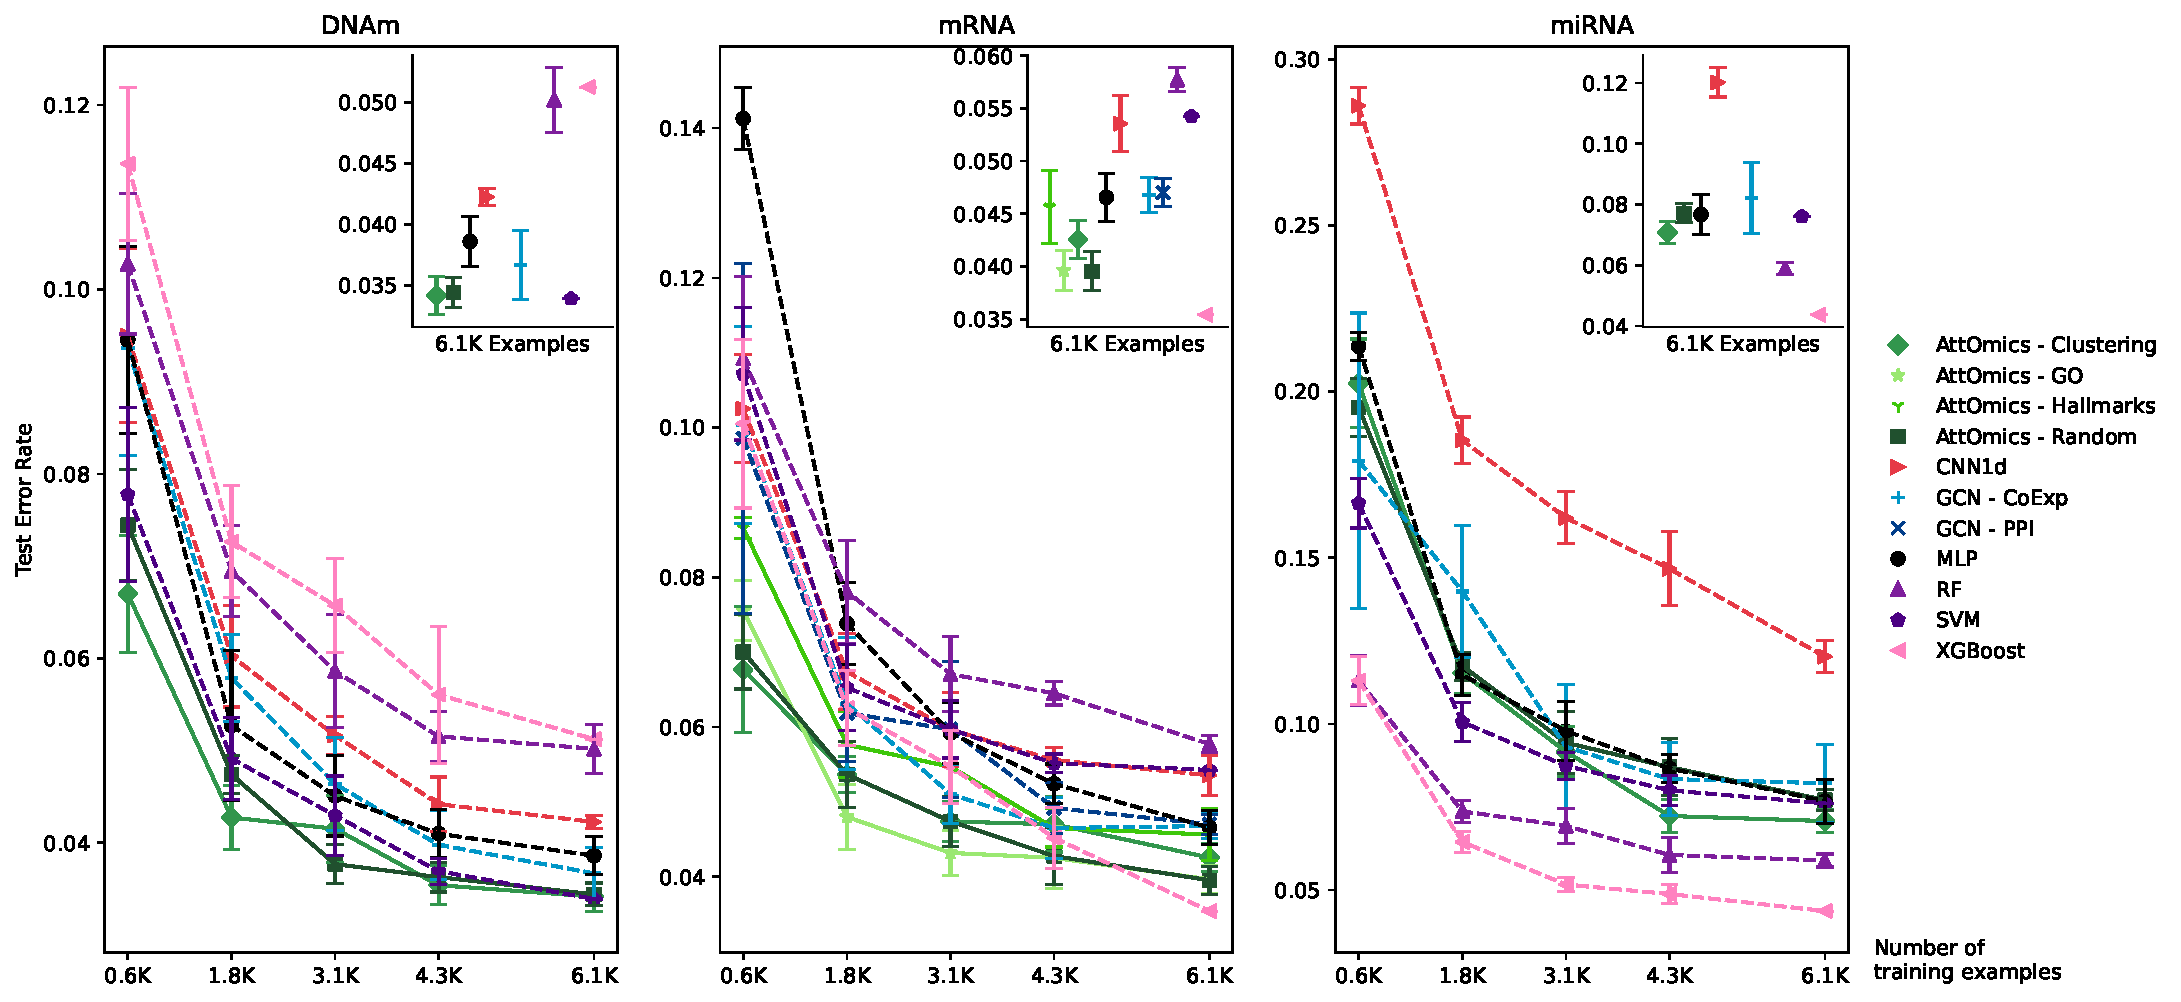
\includegraphics[width=0.9\textwidth]{Beaude.168.fig.3.pdf}
		 \caption{Error rate on the test set according to the size of the training set.}\label{fig:limit_train_classif}
	 \end{figure*}

	 Despite the broad adoption of high throughput methods in personalized medicine, the availability of omics data from cancer patients remains limited.
	 We explore the impact of the training database size on the performances of AttOmics and other deep-learning architectures by training the different models on a subset of the training set.
	 The different subsets are created by randomly sampling 10\%, 30\%, 50\%, and 70\% of the training set while preserving class proportions.
	 To prevent data leakage, structures computed from the training set, like co-expression graphs or clustered grouping, are recomputed with the selected subset.
	 For each subset, five models are trained.
	 The reported performance metrics are estimated on the test set.

	 \Cref{fig:limit_train_classif} shows the average and standard deviation of the error rate on the cancer-type classification task according to the training set size for all tested methods.
	 A wilcoxon test is used to assess the significance of the results, p-value are corrected for multiple testing with a two-stage approach describe in~\cite{10.2307/2346101}~(Table S8 in the supplementary file).
	 The best error rates are achieved with the highest number of samples.

	 CNN1d is the worst model across omics when trained on the whole training set.
	 Convolutions are more suited for structured data, and even the incorporation of a structure in the data based on the chromosomal location is a constraint that limits the range of possible interactions.
	 Only genes in the same convolution window interact with each other, which does not consider long-range interaction.
	 The AttOmics model achieves better or similar performances than the best model that does not use self-attention across the different omics.
	 For methylation data, the mean error rate is better than the GNN --- CoExp approach.
	 However, there is no statistical significance as the performances on the GNN are more variable across training.
	 For gene expression data, similar error rates are achieved between \gls{mlp} and \gls{gnn} approaches.

	 Depending on the omics, non-deep-learning models do not perform equally.
	 The \gls{svm} approach obtains similar performances for the methylation data to AttOmics, whereas \gls{xgboost} and \gls{rf} achieve lower performances than the CNN1d model.
	 \gls{xgboost} and AttOmics have the same performances for gene expression data.
	 \gls{svm} and \gls{rf} do not compete with other architectures and obtain one of the highest error-rate.
	 For the miRNA data, the best-performing methods are \gls{rf} and \gls{xgboost}.
	 The \gls{svm} approach obtains an error-rate comparable to the deep-learning architecture, and there are no differences between the different deep-learning models (Table S6 in supplementary file).

	 We do not observe a difference in terms of performances between the different grouping strategies.
	 For methylation data, random or clustering approaches give the same error rate.
	 For gene expression data, GO and random grouping reach the same error rate, whereas the clustering approach has worse performances but still performs better than other deep learning approaches.
	 The architecture based on the hallmarks grouping achieves performances similar to the \gls{mlp} or \gls{gnn}, whereas other grouping approaches improved the performance.
	 The worst performance is probably due to this strategy's implicit feature selection; only 4305 genes were used.
	 A too-large selection of the number of features limits the potential for the model to learn the relevant interactions.

	 Since, in real-world applications, datasets are much smaller than the TCGA dataset, it is particularly interesting to analyze the performances of models trained from small training sets.
	 Reducing the number of training examples affects model performance adversely, as a limited training database hinders the capacity of the model to extract hidden information during training.
	 The performances vary similarly between the different grouping strategies when reducing the number of parameters.
	 When training with the lowest number of examples, we can identify different sets of architectures.
	 For mRNA, the \gls{mlp} has the worst performance.
	 All architectures incorporating a structure in the data (\gls{cnn} and \gls{gnn}) achieve similar performances.
	 AttOmics architecture performs best and outperforms non-deep-learning methods with small training sets for gene expression and methylation data.

	 Only the hallmarks grouping strategy has worse performances than the other grouping strategies.
	 We note that for the \gls{gnn} architecture, the performances standard deviation across different training with the same number of training varies more than AttOmics architecture.
	 This suggests that the \gls{gnn} architecture depends on the selected training examples, whereas AttOmics models are less sensitive to this issue.

	 Other classification metrics were improved, such as the f1-score~(Figure S4 and Table S7 in the supplementary file).
	 The improvement is more significant when the number of training examples is limited.

	 The size of a neural network, i.e.\ its number of parameters to fit, has a strong impact on its performances and required hardware resources (memory, computing time).
	 AttOmics architecture reduces the number of parameters compared to the CNN architecture or \gls{mlp} and achieves similar or better performances (Table S6 in the supplementary file).
	 Due to the high number of features in the omics profile, most \gls{mlp} parameters are within the first layer.
	 However, the total number of parameters of a model is limited by the available hardware.
	 One way to reduce the number of parameters would be to select features, but as explained earlier, this may lead to a loss of relevant information.
	 Another approach would be to reduce the dimension of the first layer, therefore limiting the range of the possible number of neurons in the first hidden layer to meet the memory constraints.
	 Limiting the first projection's space leads to an extensive compression of the omics profile.
	 With self-attention, we can increase the dimension of the projection by reducing the number of parameters and compressing the omics profile more gradually.
	 For instance, for the mRNA clustering approach with self-attention, the profile is projected into a 43280-dimensional space with only 125 million parameters, whereas projecting into the same dimension would require 2.5 billion parameters with an \gls{mlp}.

	 As self-attention is known to have a quadratic complexity, we explored its impact on the memory usage of the model and the runtime to obtain prediction from the test set~(Figure S7 and Table S9 in the supplementary file).
	 During inference on the test set, there is a 45\% increase in memory consumption with the \gls{mlp}.
	 With AttOmics, memory overhead range from 65\% for the largest model to 250\% for the smallest model.
	 The runtime increases with AttOmics compared to the \gls{mlp} but stays in the milliseconds' range and is at least an order of magnitude better than the non-deep-learning methods.


	 A similar study is performed for prognosis prediction.
	 The evolution of the $\operatorname{C-Index}$ according to the number of training examples is presented in~Figure S6 (see supplementary file).
	 All models obtain similar performance on this task.
	 We note that the AttOmics architecture is more stable as it achieves a similar $\operatorname{C-Index}$ as the best state-of-the-art approach in different omics.
	 Indeed, for DNAm data, AttOmics has a similar $\operatorname{C-Index}$ to the \gls{cnn} architecture. For mRNA data, AttOmics has similar performances to the \gls{gnn}.
	 For miRNA data, the \gls{gnn} architecture outperforms all other architectures.

	 To conclude these results, incorporating self-attention in the architecture allows having a softer compression of the features, improving the representation of the data and, therefore, the performances.

	 AttOmics works on methylation data (DNAm) and gene expression data (mRNA) but not on micro-RNA expression data (miRNA).
	 For miRNA data, the best performances were obtained with non-deep-learning approaches.
	 There is some uncertainty when using biologically-motivated groups, as the domain knowledge constantly evolves.
	 When using biologically-aware groups, the model is limited to only considering a subset of the possible feature interactions.
	 Random or clustering grouping can detect relevant interactions not yet included in the biological knowledge.
	 Future work will investigate different biological knowledge.
	 Nevertheless, in the present paper, one can prefer biologically-motivated groups that are more interpretable, although the other grouping strategies give slightly better results.
	 This reflects the well-known trade-off between performance and interpretability in machine learning~\cite{Linardatos2021_ExplainableAI}.

 \subsection{Attention map interpretation}

	 \begin{figure}[htbp]
		 \centering
		 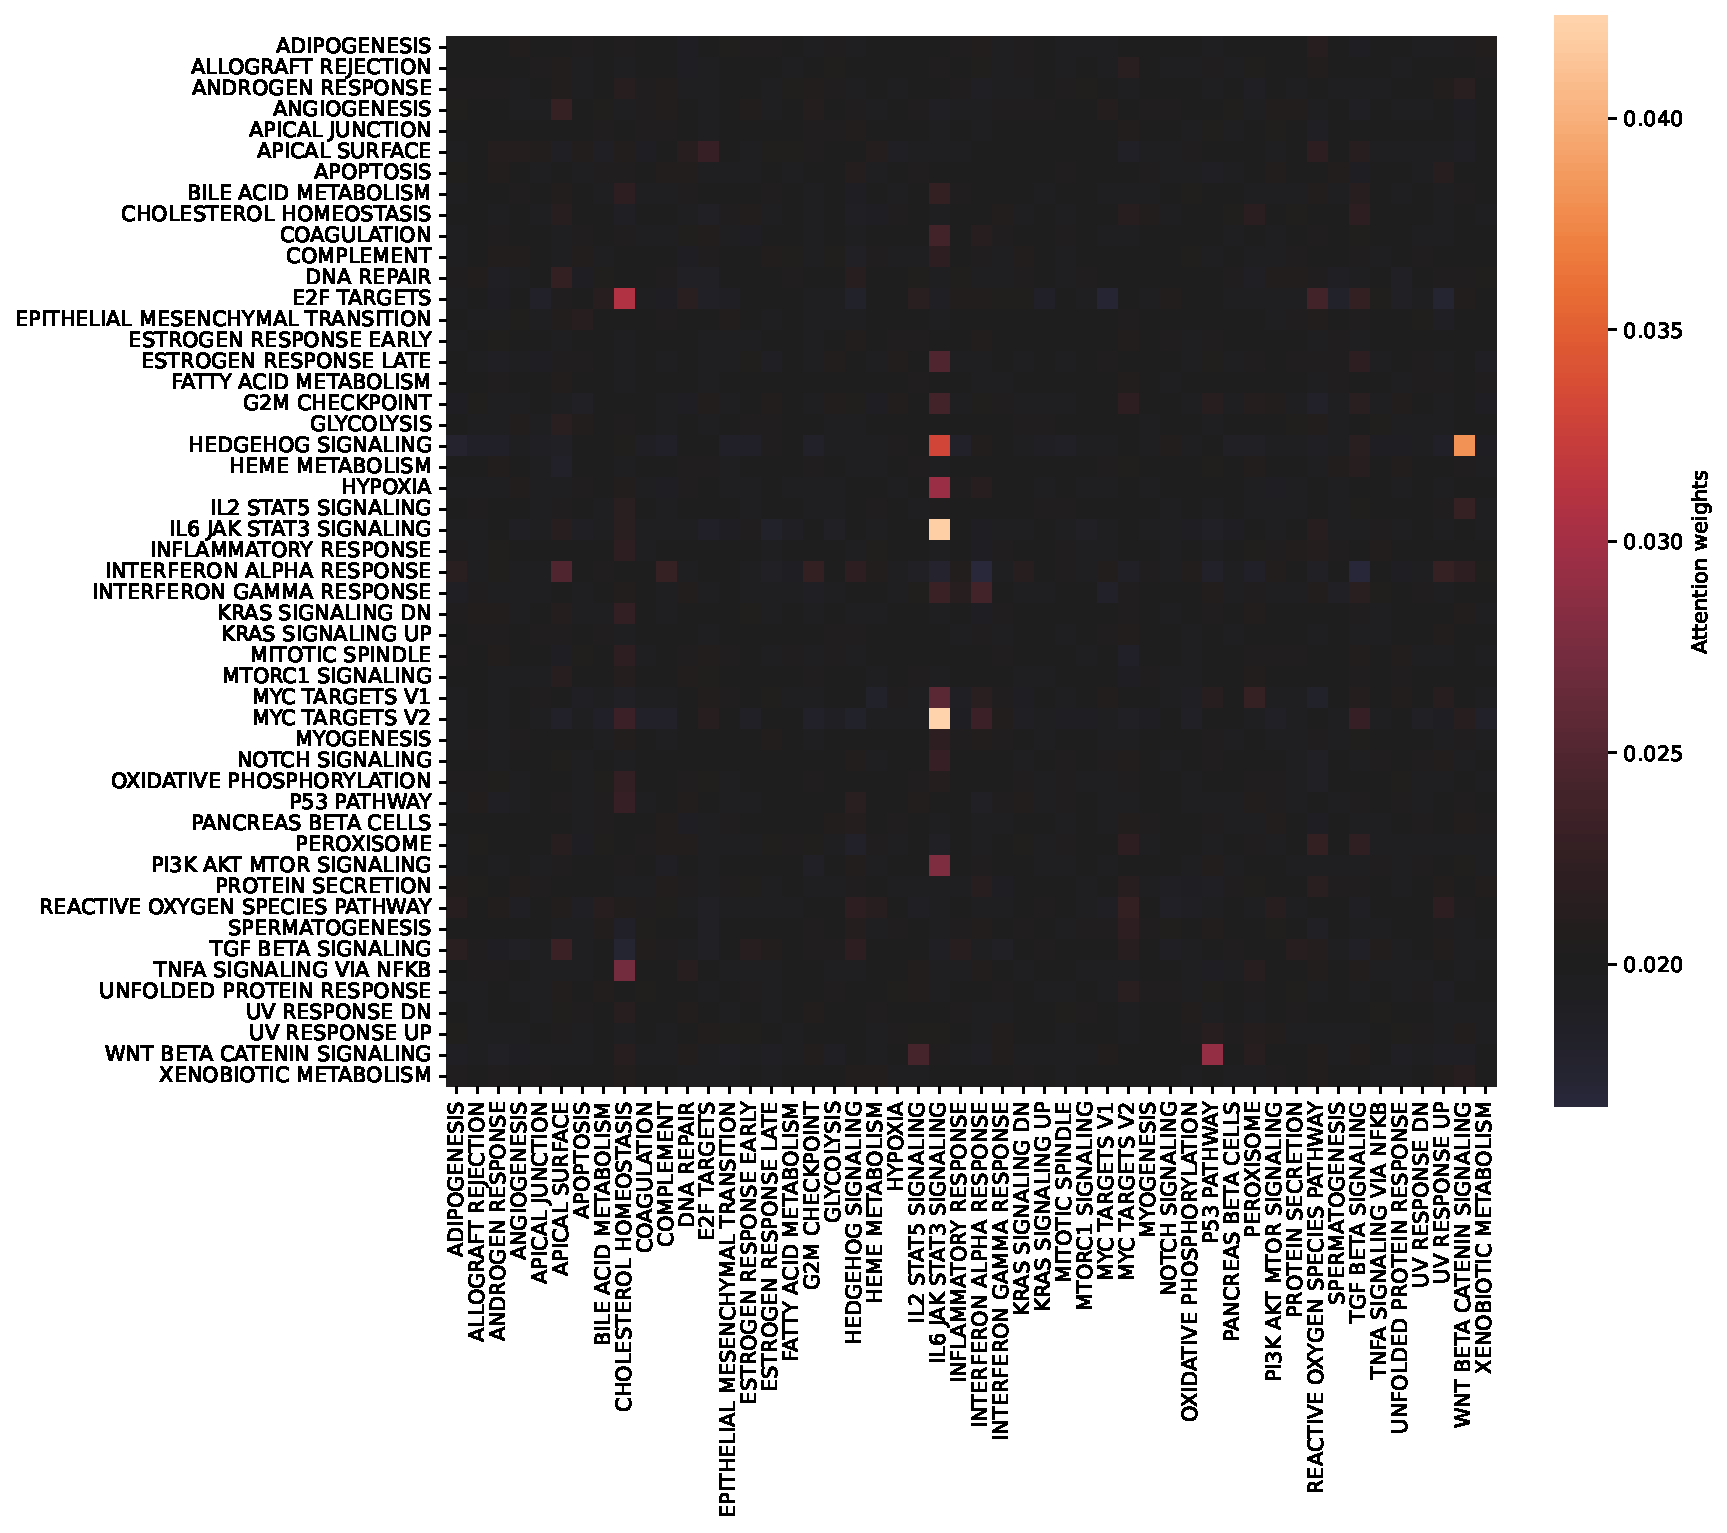
\includegraphics[width=\linewidth]{Beaude.168.fig.4.pdf}
		 \caption{Attention map visualisation for the TCGA-CESC class obtained after applying the hallmarks grouping on \gls{mrna}.}\label{fig:att_map_viz}
	 \end{figure}

	 One advantage of using self-attention in the model is the ability to visualize the learned interactions~(\cref{fig:att_map_viz}).
	 The attention map corresponds to the attention weights average across patients with the same phenotype.
	 The learned interactions are different across cancer~(Figure S9 and Figure S10 in supplementary file), suggesting that the model learns interactions specific to each cancer.

	 The self-attention mechanism used in the architecture was not designed to be an interpretability tool.
	 However, it can provide information on the interaction learned by the model depending on the grouping strategy.
	 We used GO slim or MSigDB hallmarks as a biological knowledge-aware grouping strategy.
	 The terms used in GO slim represent general biological processes; the high level of the terms makes it difficult to link the detected interaction with the phenotype.
	 On the contrary, MSigDB hallmarks focuses on important and specific biological processes and  are, therefore, easier to interpret.


	 With the hallmarks grouping, we identified interactions between well-known pathways in cervical cancer: Wnt signaling, HedgeHog signaling, and JAK/STAT signaling~(\cref{fig:att_map_viz}).
	 STAT proteins play a role in the development of cervical cancer~\cite{gutierrez-hoyaRoleJAKSTAT2020}.
	 The inactivation of the Wnt pathway is known to promote cell growth in cervical cancer~\cite{yangWntSignalingCervical2018}.
	 It has been shown that HedgeHog pathway components are expressed in cervical cancer cells and are involved in cell proliferation~\cite{samarzijaHedgehogPathwayRegulators2012}.
	 It has also been shown that there is a crosstalk between Wnt and HedgeHog pathways, which are known to be involved in chemo-resistance in cervical cancer~\cite{kumarRoleNotchHedgehog2021}.


	 Interestingly, we identified similar interactions learned by the model between the GO slim and hallmarks grouping strategies.
	 For BLCA cancer, a model based on GO slim identified multiple interactions involved in the inflammatory response (GO:0006954).
	 In the model based on hallmarks, the inflammatory response group is also identified as involved in different interactions~(Figure S11 in supplementary file).
	 The group composition between the two strategies is different, with an overlap of 29\%.


	 The model can handle any grouping, handcrafted groups, or based on a different knowledge source that could be used to improve the information contained in an attention map.

\end{document}
